%!TEX root = ../main.tex
%Adding the above line, with the name of your base .tex file (in this case "thesis.tex") will allow you to compile the whole thesis even when working inside one of the chapter tex files
%: ----------------------- introduction file header -----------------------
\onehalfspacing
\chapter{Introduction}
\label{chap:intro}
\section{The Sun}
The Sun is our nearest star and the centre of our solar system. It is a G2 type star located on the main sequence of the Hertzsprung Russell diagram. It has a luminosity of $(3.84 \pm 0.04) \times 10^{26}$ W and a radius R$_\odot = (6.959 \pm 0.007) \times 10^8$ m. With a mass of $(1.9889 \pm 0.0003) \times 10^{30}$ kg, the Sun comprises $>$ 99\% of the solar system's total mass \citep{Foukal2004}. Formed from a cooling cloud of gas and dust 4.6 billion years ago, the Sun now has a core with a temperature of 15 MK, which enables nuclear fusion to occur. %There are a number of nuclear fusion processes in the Sun's core, the most common of which is the proton-proton or `pp' chain whereby four protons collide and fuse to form a Helium nucleus. The most frequent pp chain is known as ppI, it occurs 86\% of the time \citep{Turck-Chieze2011} and is as follows,
% $$
% ^1_1\mbox{H} + ^1_1\mbox{H} \rightarrow ^2_1\mbox{H} + e^+ + \nu_e
% $$
% $$
% ^2_1\mbox{H} + ^1_1\mbox{H} \rightarrow ^3_2\mbox{He} +\gamma
% $$
% $$
% ^3_2\mbox{He} + ^3_2\mbox{He} \rightarrow ^4_2\mbox{He} +2^1_1\mbox{H}
% $$
% Here, $^1_1\mbox{H}$ is a proton or Hydrogen nucleus, $^2_1\mbox{H}$ is its isotope Deuterium, $^3_2\mbox{He}$ is the Helium isotope Triteum, $^4_2\mbox{He}$ is Helium, $e^+$ is a positron, $\nu_e$ is an electron neutrino and $\gamma$ is a gamma ray photon. A complete ppI chain releases $4.2 \times 10^{-12}$ J of energy in the form of electromagnetic radiation. The energy output of all pp chains account for 98.8\% of the total energy produced by the Sun \citep{Turck-Chieze2011}. 

% Photons generated in the ppI travel outwards from the core however, their small mean free path of 0.9cm means that this takes on the order of $10^5$ years to reach the solar surface \citep{Mitalas1992}. At 70\% of the Sun's radius (0.7 R$_{\odot}$), the temperature has cooled to 1 MK thereby allowing electrons to bind to atomic orbitals, drastically decreasing the scattering rate of photons. Energy transfer from here to the solar surface at 1 R$_{\odot}$ is now primarily done through convection. 

The layer of the Sun at 1 R$_{\odot}$ is known as the photosphere and is what would be called the surface of the Sun.
%This is the point at which the optical depth for visible light photons is 1 and their mean free path is much greater than the distance between scattering centres on the solar surface. 
Above the photosphere is the Sun's atmosphere consisting of the chromosphere, transition region and the corona. Figure \ref{fig:Sun} shows the interior layers of the Sun and its atmosphere.
\begin{figure}[t]
    \centering
    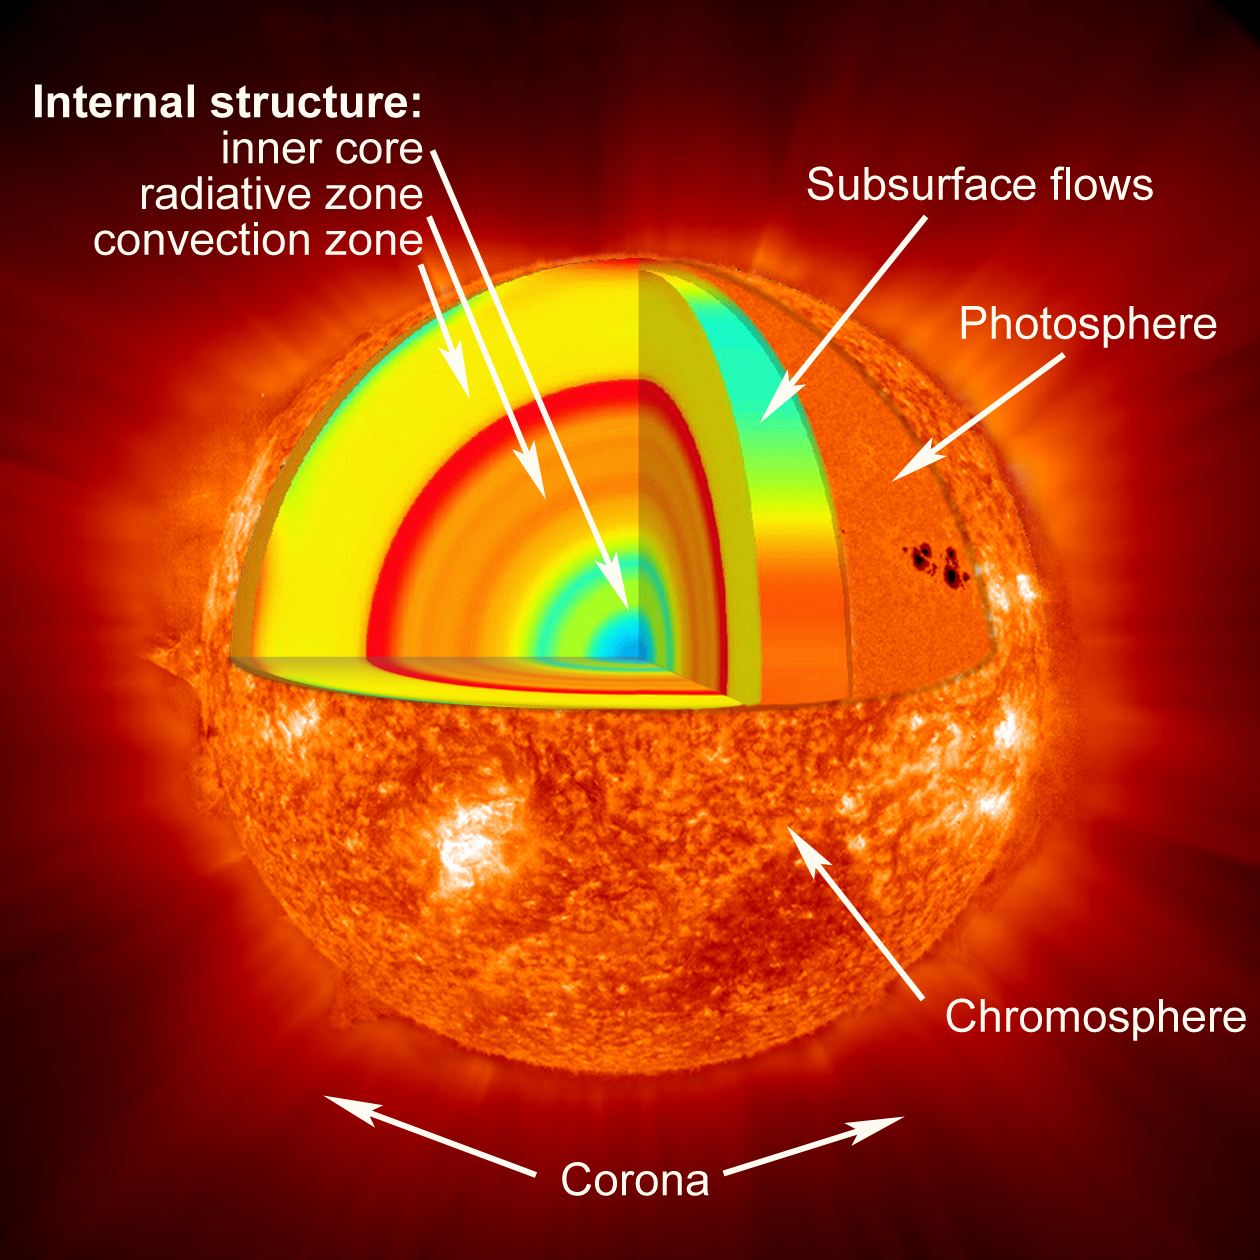
\includegraphics[width=0.5\columnwidth]{Images/Sun_interior.jpg}
    \caption[Diagram of Sun's interior and atmospheric layers.]{Diagram of Sun's interior and atmospheric layers. Photons produced by nuclear fusion in the core transfer energy outwards through the radiative zone to ~0.7 R$_{\odot}$. At this point, convection becomes the main form of energy transport. The visible surface of the Sun is known as the photosphere and marks the boundary between the interior and the atmosphere. The solar atmosphere consists of three layers, the chromosphere, the transition region (not shown) and the corona.}
    \label{fig:Sun}
\end{figure}

\subsection{The Corona}
%Perhaps the most interesting part of the Sun, for this PhD student at least, is the outermost layer of the solar atmosphere, the corona. 
The outermost layer of the solar atmosphere is called the corona. It is a hot, tenuous plasma which displays a number of interesting phenomena thought to be governed by its complex magnetic field. The corona begins $\sim 2500$ km above the photosphere after a layer in the Sun's atmosphere known as the transition region, where electron density decreases and temperature increases dramatically (Figure \ref{fig:corona_temp}). The electron density in the corona ranges from $10^{9} \mbox{ cm}^{-3}$ at the base to $10^{6} \mbox{ cm}^{-3}$ at distances of 1 R$_{\odot}$ from the solar surface. Densities vary throughout the corona. Sparse, underdense regions at the base of the corona known as coronal holes exhibit densities of $\sim ( 0.5 - 1.0) \times 10^8 \mbox{ cm}^{-3}$ whereas areas of high magnetic activity known as active regions have electron densities of $\sim 2 \times 10^9 \mbox{ cm}^{-3}$.%Certain areas in the corona however, exhibit electron densities approximately an order of magnitude greater than the ``quiet Sun". Theses areas of high electron densities ar 
\begin{figure}
    \centering
    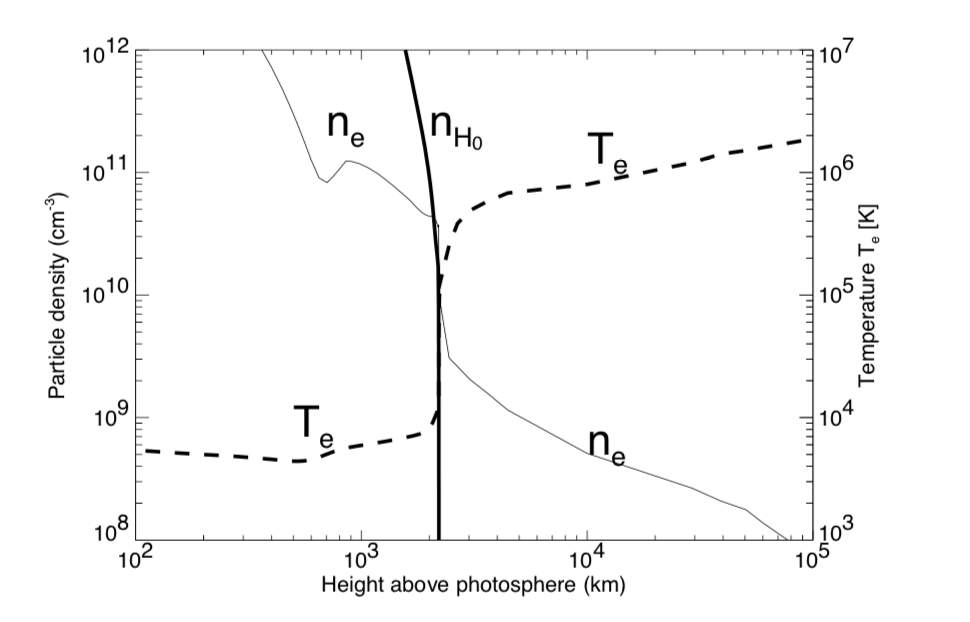
\includegraphics[width=0.75\columnwidth]{Images/Corona_temp.png}
    \caption[Model of electron density and temperature with height in the solar atmosphere.]{Model of electron density and temperature with height in the solar atmosphere. The region around 2000 km showing a sharp rise in temperature and sharp fall in electron density is known as the transition region, above this height plasma becomes fully ionised. Image taken from \cite{Aschwanden2004}}
    \label{fig:corona_temp}
\end{figure}%Puzzlingly however the temperature over this range increases to the order of 1MK. This ``coronal heating problem" remains unexplained and is one of the main poeices of understanding lacking form solar physics.

%Historically, the corona could only be observed during total solar eclipses as the emission from the corona due to Thompson scattering is far less intense than emission from the photosphere. 
Observing the white light corona is done with a number of ground-based and space-based instruments called coronographs, that emulate the effect of a total eclipse. The Large Angle and Spectrometric Coronagraph (LASCO) on board the Solar and Heliospheric Observatory (SOHO) is one such instrument and allows the corona to be observed from distances of 2-32 R$_\odot$. %This has lead to an increase in observations of structures known as coronal streamers and the phenomenon of Coronal Mass Ejections (CMEs). %Due to its high temperature, the corona is easily visible in extreme ultraviolet (EUV) light and is observed in many different passbands with instruments such as the Atmospheric Imaging Assembly (AIA) on board the Solar Dynamics Observatory (SDO). 
%Solar flares, a release of vast amounts of energy due to reconnection of magnetic field lines in the corona, are some of the most energetic events in the solar system. During solar flares magnetic structures known as coronal loops fill with hot plasma and begin to emit in soft X-rays. At the same time, electrons are accelerated towards the solar surface where their energy is converted to hard X-rays in the collision via bremsstrahlung. These X-ray observations of the corona have been taken by the Reuven Ramaty High Energy Solar Spectroscopic Imager (RHESSI).

Energetic events in the corona such as solar flares and coronal mass ejections (CMEs), described in \ref{subsec:sf} and \ref{subsec:CMEs}, are studied across the electromagnetic spectrum. They are studied in order to understand how particles are accelerated, how energy is released and ultimately, why the corona has such an unaccountably high temperature.
Most particle acceleration events in the solar corona have a diagnostic in radio spectra. This PhD focuses on studying these radio diagnostics at their highest temporal and spatial resolutions to date.
%Some of the most energetic phenomena in the solar system occur due to magnetic field configurations in the corona. Solar flares, coronal mass ejections and solar energetic particles all involve the acceleration of particles into the heliosphere and can often impact Earth. Studies of these phenomena have been carried out across the electromagnetic spectrum however the main interest in this PhD is radio phenomena.


% and like all stars is supported by nuclear fusion of hydrgoen in its core. Photons produced in this nuclear furnace travel oytwards, bwing scattered many millions of times on the way until they reach the photosphere. Here the optical depth of the is 1 where the mean free path of a photon is much greater than the scattering  scattering distance so they escape to space.

\subsection{Solar Flares}
\label{subsec:sf}
Solar flares are massive releases of magnetic energy commonly believed to be due to a reconfiguration in the complicated magnetic field structure in an active region.  They are some of the most energetic events in the solar system, releasing $\sim 10^{25}$ J of energy over a matter of minutes. Flares are observed across the electromagnetic spectrum from radio waves to $\gamma$ rays with energies $> 10$ MeV. They are classified by the amount of X-ray flux (W m$^{-2}$) detected by the Geostationary Operational Environmental Satellite (GOES) 1-8 {\AA} band on a logarithmic scale as being A, B, C, M or X class with A being the lowest flux ($10^{-8} \mbox{ W m}^{-2}$) and X the highest ($10^{-4} \mbox{ W m}^{-2}$). Each class is further subdivided into a linear scale.
A timeseries of X-ray flux from a solar flare is often called a lightcurve and has three characteristic phases; a pre-flare phase which shows X-ray flux associated with the active region where the flare occurs, an impulsive phase showing a sharp rise in X-ray flux corresponding to accelerated particles colliding with the solar surface, and a gradual decay phase where plasma heated by the flare gradually cools back to its pre-flare state. Figure \ref{fig:GOES_Xclass} shows a GOES light curve of the X9 class flare that occurred on 2017-09-10 and the three flare phases described above.

%It shows a characteristic impulsive rise of flux followed by a gradual decay back to the background level of flux.

\begin{figure}
    \centering
    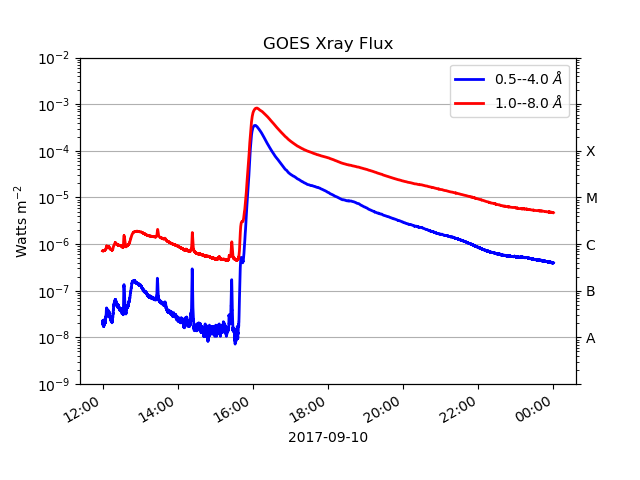
\includegraphics[width=0.75\columnwidth]{Images/GOES_Xclass.png}
    \caption[GOES lightcurve for X9 class flare on 2017-09-10]{The GOES lightcurve of the X9 flare that occurred on 2017-09-10. The red curve shows the 1-8 {\AA} channel by which the flare is classified while the blue curve shows the 0.5-4 {\AA} band. The three characteristic phases of a solar flare are clearly displayed here. The pre-flare phase before $\sim 16:00$ UTC, the impulsive phase indicated by the sharp rise in flux and the gradual decay phase where X-ray flux gradually returns to the pre-flare level.}
    \label{fig:GOES_Xclass}
\end{figure}
During solar flares, magnetic structures known as coronal loops fill with hot plasma and begin to emit in soft X-rays. At the same time, electrons are accelerated towards the solar surface where their energy is converted to hard X-rays in the collision via bremsstrahlung. %These X-ray observations of the corona have been taken by the Reuven Ramaty High Energy Solar Spectroscopic Imager (RHESSI).

\subsection{Coronal Mass Ejections (CMEs)}
\label{subsec:CMEs}
In certain magnetic reconnection events, plasma suspended in a magnetic flux rope erupts from the corona into the heliosphere, the volume around the Sun where the interplanetary medium is dominated by particles flowing outward from the Sun. These eruption events are known as coronal mass ejections and accelerate 10$^{15}$ g of charged particles at typical speeds of up to $\sim 2500 \mbox{ km s}^{-1}$ \citep{Gopalswamy2000}. A ``textbook" CME structure consists of a bright front that surrounds a dark cavity and a bright central core. CMEs are observed using coronographs as they are much fainter than the solar disk. An example of a CME observed using the LASCO C2 corona with a field of view from 1.5 R$_\odot$ to 6 R$_\odot$ can be seen in Figure \ref{fig:CME}. Ejected material from a CME can interact with the Earth's magnetosphere and are known to have caused adverse effects including satellite communication disruption, radio blackouts, wide spread power outages and large inaccuracies in GPS postions. CMEs can travel faster than local Alfv\'{e}n speed in the corona leading to a shock which can accelerate particles. 

\begin{figure}
    \centering
    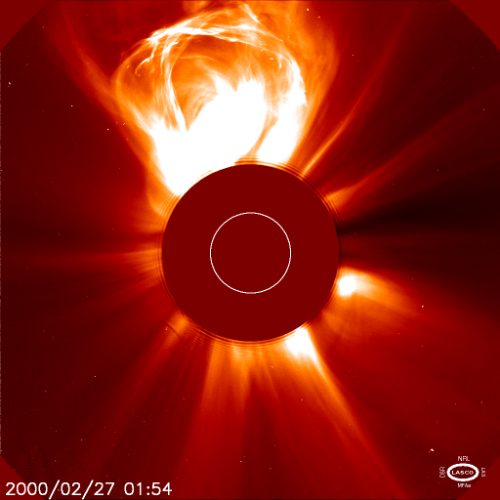
\includegraphics[width=0.5\columnwidth]{Images/LASCO_C2_CME.jpg}
    \caption{CME observed with the LASCO C2 instrument on 2000-02-27. The blank area shows the extent of the coronograph and the white circle represents the solar disk.}
    \label{fig:CME}
\end{figure}


%\section{Solar Radio Emission}
%Most of the interesting things in the Sun at radio wave lengths are due to a variety of plasma emission processes that are observed as bursts in dynamic spectra. The frequency span and duration of these bursts are often the defining characteristics that categorise these bursts into 5 types. Of particular interest are Type III burst which occur due to Langmuir wave interactions in the solar corona.
%and are discussed in greater detail at some point. 
%These bursts are thought to originate from accelerated electrons from a flaring region in the Sun and as such can inform us about the process that allows vast amounts of energy release in a solar flare.
%Radio emission from the Sun is typically unimpressive. It is mostly due to low energy bremstrahlung radiation of electrons far from the scattering centre. There are a number of pheneomena however, who's brightness temperatures far exceed that if the quiet Sun that are topics of great interest in the Solar community. These include Type I-V radio bursts described by \cite{Wild1950}
%Due to its complicated magnetic structure, the solar corona is home to a number of sites of particle acceleration. 


\section{Solar Radio Bursts}
Particles in the solar corona are accelerated by solar flares and CMEs, resulting in a range of radio bursts distinguish in spectra as the ``classic" Type I-V radio bursts described by \cite{Wild1950}. A wealth of other fine structure radio bursts are also observed, predominantly found in radio storms such as S bursts, drift pairs and stria \citep{McConnell1980,Melrose1982,NelsonandMelrose1985}. 
 The fine structure of these bursts can often reveal information about small-scale turbulence in the corona \citep{Kontar2017} and offer the greatest chance of solving the coronal heating problem.
 %which have been linked to features and events in the solar atmosphere i.e., active regions and coronal shocks \citep{Dulk1985, NelsonandMelrose1985}. There are 

%Understanding the temporal and spatial structure of these bursts help us understand more about particle acceleration and energy release in the solar corona and may give insight into the coronal heating problem.

A brief description of some solar radio phenomena is given here while a more in depth review of the plasma emission process is given in appendix \ref{app:plasma}.
\begin{figure}
    \centering
    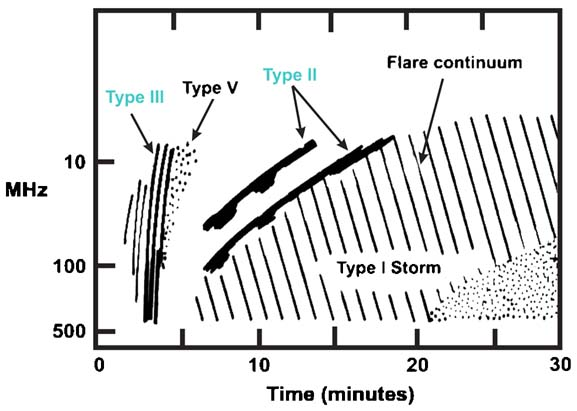
\includegraphics[width=0.75\columnwidth]{Images/Burst_cartoon.jpg}
    \caption[Cartoon of Type I-V radio bursts]{A cartoon of Type I-V radio bursts. Image taken from \cite{Cliver2009}}
    \label{fig:burst_cartoon}
\end{figure}
\paragraph{Type I bursts}
Type I emission can appear as bursts and/or a continuum originating from ``storm centres" that are associated with active regions. Type I storms can last for many days. Emission from Type I bursts is highly circularly polarised in the o-mode (whereby light is circularly polarised in the same direction as electrons gyrating about a magnetic field line) and is also particularly directional with an increase in intensity as active regions rotate to the centre of the disk. Unlike Type II or III bursts, they do not exhibit a harmonic structure.
\paragraph{Type II bursts}
Type II radio bursts are a form of radio emission seen from the Sun and are identified by a slow ($\sim 0.1$ MHz s$^{-1}$) drift to lower frequencies in dynamic spectra. The frequency drift can be used to find the velocity of the shock causing a burst if the electron number density as a function of height is known. The velocities of Type II bursts are often found to be $\sim 1000 \mbox{ km s}^{-1}$, much faster than the Alfv\'{e}n velocity in the quiet corona, $\approx 270 \mbox{ km s}^{-1}$, meaning a shock must be present. Other basic properties of Type II bursts include:
\begin{enumerate}
    \item Narrow bandwidths of up to $\sim 100$ MHz from initial to final frequencies.
    \item A harmonic structure of two bands with a frequency ratio slightly less than 2:1 at a fundamental, $f_p$, and harmonic, $2f_p$, frequency can be seen for most Type II bursts. This structure is consistent with the idea that Type II emission is due to plasma oscillations.
    \item A large number of Type II bursts contain band splitting into an upper and lower band for each of the harmonics in their spectra. The cause for this splitting is not fully understood but it is commonly thought that the two bands are related to emission upstream and downstream of the MHD shock front which causes the Type II burst \citep{Smerd1974,NelsonandMelrose1985, Vrsnak2002}.
    \item Herringbone structure. Approximately 20\% of Type II bursts show a herringbone structure of rapidly drifting emission spikes shooting out of the ``backbone" of the main frequency drift to higher and lower frequencies. These herringbones are thought to be due to electron beams being accelerated at the associated shock for the Type II burst \citep{Mann1995}. While the backbone is poorly polarised, the herringbones have been found to be quite strongly, $\sim 70\%$, polarised. This is further evidence that herringbone structure is due to Type III-like emission from accelerated electron beams.
    \item Starting emission frequencies of the order of a few 100 MHz ending at frequencies above 20 MHz. This being said, Type II burst with starting frequencies of $\sim 100$ kHz have also been observed. 
    These lower frequency bursts are thought to be due to interplanetary shocks whereas higher frequency bursts are considered to be from shocks in the low corona.
    \item Typical durations of 5-15 minutes. Type II bursts that occur after a flare do so with a delay ranging from 2-20 minutes. Bursts with shorter durations generally have higher starting frequencies. %Timing and duration    
\end{enumerate}
 
Based on these and a number of other properties discussed in greater detail by \cite{NelsonandMelrose1985}, Type II radio bursts can be used as indicators for MHD shocks in the solar corona. Observational proof of frequency varying inversely with time in the solar wind, consistent with radiation being generated at $f_p$ and $2f_p$ directly upstream from a CME-driven shock, was found by \cite{Reiner1997} and solidifies this argument.

\paragraph{Type IV burst}
Type IV bursts come in at least three sub-types with the general characteristic that they are of the from of broadband emission lasting for several hours. Early stationary Type IV bursts (also known as the flare continuum) associated with the decay phase of solar flares, late stationary bursts which appear similar to Type I emission, and moving Type IV bursts which exhibit a smooth, wide-band spectrum.
\paragraph{Type V burst}
The last of the broadband emission bursts, Type V radio bursts typically have a duration of 1-3 minutes and appear as an afterglow from Type III bursts. Type V emission is strictly less than 150 MHz and is accepted that it results from electrons that generate a Type III burst and become trapped in a closed magnetic loop in the corona.

\paragraph{Fine Structure: S bursts} 
S bursts, initially called Fast Drift Storm (FDS) bursts, were first observed at the Culgoora Solar Observatory in 1967 \citep{Ellis1969} They were later renamed by \cite{McConnell1980} who likened them to Jovian S bursts. They have a narrow bandwidth of the order of 0.03 MHz and a drift rate of 1-2 MHz s$^{-1}$ and durations much less than 1s. \cite{McConnell1980} also concluded that S bursts are radiated at either the plasma frequency or its harmonic in a manner similar to Type III bursts, see appendix \ref{app:plasma}, but that the implications of S burst fine structure and coronal scattering can only be defined once it is determined which harmonic of the plasma frequency they are radiated at. \cite{Melnik2010} propose a model of S bursts being generated by coalescence of fast magnetosonic waves with Langmuir waves which agrees well with the analysis of \cite{Clarke2019}. Modern observations of S bursts, such as those conducted using LOFAR's tied-array imaging mode \citep{Morosan2015}, can give greater insight into the spectral and temporal variability of S bursts and what this might mean for the environment they are generated in.

%where S stands for ``short" or ``storm", are balch blah blhs . First described by \cite{McConnell1980}, they are so called due to their similarity with Jovian S bursts.
\subsection{Type III Bursts}
\label{characteristics} %(This is what they look like)}\label{characteristics}
Type III bursts are possibly the most useful radio burst for studying various aspects of the corona outlined later. Furthermore, section \ref{sec:event} describes a Type III burst that is being analysed as part of this PhD.
\cite{Reid2014} review a number of notable properties of Type III bursts. The defining characteristic of Type III bursts is a drift from high to low frequencies in a dynamic spectrum. The drift rates for Type III bursts are typically quite fast, of the order of $\sim$ 10 MHz s$^{-1}$ depending on the frequency. The frequency drift rate, $df/dt$, has been found to have various relations with frequency \citep{Reid2014} but most are agree that $df/dt \propto f^{\alpha}$, where $\alpha$ varies depending on the study from $\sim 1$ to $\sim 2.7$. 

\cite{Ginzburg1958} proposed that Type III bursts are emitted at the plasma frequency,
\begin{equation}\label{eq:1}
    \omega_{p}^2 = \frac{n_ee^2}{m_e \varepsilon_0}
\end{equation}
where $n_e$ is the number density of electrons, $m_e$ is the electron mass, $e$ is the electron charge and $\varepsilon_0$ is the permittivity of free space.
Although Eq. \ref{eq:1} is relatively simple, it contains an important principle of plasma physics. Namely, the plasma frequency is proportional to the square root of the electron density. This means that plasmas at higher electron densities will oscillate at higher frequencies than those of lower densities. The drift in Type III bursts, which are emitted at $\omega_p$, is therefore an indication of the emission source moving from an area of high electron density, the photosphere, to low density, the upper corona.

Type III bursts are observed to be in two bands, a fundamental and harmonic band that are emitted at $\omega_p$ and $2 \omega_p$ respectively. Both bands exhibit the same frequency drift although the flux of the harmonic band is usually less than that of the fundamental band. The process of plasma emitting radio frequencies at $\omega_p$ and $2 \omega_p$ will be explained in more detail in section \ref{Plasma Emission}. 
%Type III bursts can be identified from dynamic spectra as short periods of high intensity drifting quickly $\sim$ 10 MHz s$^{-1}$ from high to low frequency.

\begin{figure}
    \centering
    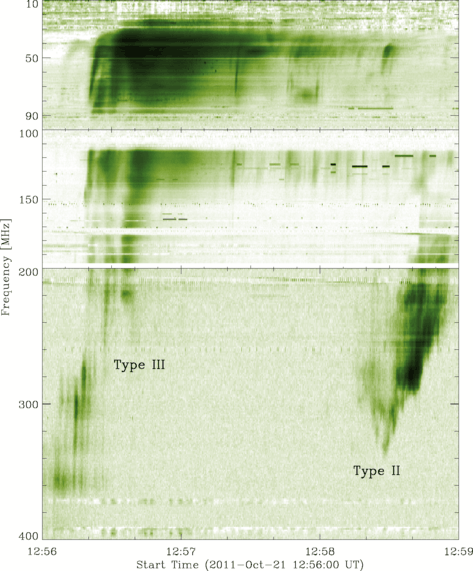
\includegraphics[width=0.5\columnwidth]{Images/Pietro_typeIII.png}
    \caption[A number of Type III bursts observed by \cite{Zucca2012} on 21 October 2011.]{A number of Type III bursts observed by \cite{Zucca2012} on 21 October 2011. Note the Type III storm below 200 MHz and the Type II burst between 140 and 330 MHz.}
    \label{fig:bursts}
\end{figure}

Figure \ref{fig:bursts} shows Type III radio bursts below 400 MHz observed by \cite{Zucca2012}. A Type II burst was also observed between 140 and 330 MHz and exhibits a much slower frequency drift than the Type III bursts. A Type III storm can be seen below 200 MHz. This is when Type III emission is continuous over the span of large time scales and can last days. Type III bursts come in a number of subcategories described below.

%\subsection{Sub-categories of Type III Bursts} %(Here's some different types)}
%here are different subcategories of Type III bursts. These include: reverse and bi-directional bursts, Type IIIb bursts, U and J bursts.

\paragraph{Reverse and bi-directional bursts}
A typical Type III burst is produced when an electron beam travels along a magnetic field line away from the Sun to areas of lower density. During the magnetic reconnection process that accelerates these electrons, some electrons travel towards the Sun to areas of higher density and thus have a reversed frequency drift. Bursts where both the regular and reverse drifts can be seen simultaneously are bi-directional bursts.

\paragraph{Type IIIb bursts}
While typical Type III bursts have smooth emission, Type IIIb bursts contain a fragmented substructure. This substructure is in the form of a chain of emission bands/striae that drift in frequency as a whole but individually show little frequency drift.

\paragraph{Type U and J bursts}
In the case where electrons are travelling along a closed magnetic field line, a turning point in the frequency drift of a Type III burst can be observed. For electrons that generate radio emission down to the footpoint of the magnetic field line, a U burst is observed. A U burst can be identified as an inverted U on a dynamic spectrum. More often, electrons stop generating radio emission as they travel back down the magnetic field line so only the turning point in frequency drift is visible in dynamic spectra. These are known as J type bursts. The reason for higher occurrence of J bursts compared to U bursts is described by \cite{Reid2017}.



%Intro from \cite{McConnell1980} stuff from \cite{Morosan2015} and Brendan
%\subsubsection{Drift Pairs}
%\cite{Melrose1982}

\subsection{Source Sizes in the Corona}
Analysis of short temporal bursts with small bandwidths suggest source sizes in the corona to be of the order $\sim 6000$ km \citep{McConnell1980}. Radio images of the Sun at metric and decametric wavelengths have yet to reveal this level of spatial structure. This is mostly due to the limit of resolution obtainable with modern interferometers however, the suggestion that there is a fundamental limit imposed upon the level of resolution obtainable by scattering in a turbulent corona \citep{Bastian1994} has gathered a following in recent years \citep{Kontar2017}. \cite{Riddle1974} described the effect of scattering in a spherically symmetric corona with random isotropic inhomogeneities with and without density enhancements due to streamers. Here they showed that the ``directivity pattern", the ratio of the power received from a source with and without scattering, was significantly broadened for radio bursts near the local plasma frequency, 80 MHz in their case.
Sub-arcminute interferometric observations of Type III radio bursts could give a definitive answer to this question.

%\subsubsection{Type II Radio Bursts}
% Type II radio bursts are a form of radio emission seen from the Sun and are identified by a slow ($\sim 0.1$ MHz s$^{-1}$) drift to lower frequencies in dynamic spectra. The frequency drift can be used to find the velocity of the shock causing a burst if the electron number density as a function of height is known. The velocities of Type II bursts are often found to be $\sim 1000 \mbox{km s}^{-1}$, much faster than the Alfv\'{e}n velocity, $\approx 270 \mbox{km s}^{-1}$ in the quiet corona meaning a shock must be present. Other basic properties of Type II bursts include:
% \begin{enumerate}
%     \item Narrow bandwidths of up to $\sim 100$ MHz from initial to final frequencies.
%     \item A harmonic structure of two bands with a frequency ratio slightly less than 2:1 at a fundamental, $f_p$, and harmonic, $2f_p$, frequency can be seen for most Type II bursts. This structure is consistent with the idea that Type II emission is due to plasma oscillations.
%     \item A large number of Type II bursts contain band splitting into an upper and lower band for each of the harmonics in their spectra. The cause for this splitting is not fully understood but it is commonly thought that the two bands are related to emission upstream and downstream of the MHD shock front which causes the Type II burst \citep{Smerd1974,NelsonandMelrose1985, Vrsnak2002}.
%     \item Herringbone structure. Approximately 20\% of Type II bursts show a herringbone structure of rapidly drifting emission spikes shooting out of the ``backbone" of the main frequency drift to higher and lower frequencies. These herringbones are thought to be due to electron beams being accelerated at the associated shock for the Type II burst \citep{Mann1995}. While the backbone is poorly polarised, the herringbones have been found to be quite strongly, $\sim 70\%$, polarised. This is further evidence that herringbone structure is due to Type III-like emission from accelerated electron beams.
%     \item Starting emission frequencies of the order of a few 100 MHz ending at frequencies above 20 MHz. This being said, Type II burst with starting frequencies of $\sim 100$ kHz have also been observed. These low frequency burst are thought to be due to interplanetary shocks whereas the higher frequency bursts are considered to be from shocks in the low corona.
%     \item Typical durations of 5-15 minutes. Type II bursts always occur after a flare with a delay ranging from 2-20 minutes. Bursts with shorter generally have higher starting frequencies. %Timing and duration    
% \end{enumerate}
 
% Based on these and a number of other properties discussed in greater detail by \cite{NelsonandMelrose1985}, Type II radio bursts can be used as indicators for MHD shocks in the solar corona. Observational proof of frequency varying inversely with time in the solar wind, consistent with radiation being generated at $f_p$ and $2f_p$ directly upstream from a CME driven shock, was found by \cite{Reiner1997} and solidifies this argument.

% There have been several mechanisms proposed for the acceleration of electrons at the shock front for them to produce the radio emission observed, most of which explain electrons gaining energy by scattering back and forth across the shock and being accelerated each time.


 

% \label{sec:typeIII}
% In 1942 while Britain was on the look out for radar signals of enemy aircraft, a strong, noise like and highly variable signal was noticed by radar operators. Initially it was thought that Germany had managed to learn the secret of radar and create some sort of jamming device. On further investigation it was found that this jamming was in fact radio emission from the Sun. The discovery of this radio emission being associated with a major solar flare was kept secret until after the war and was published by \cite{Appleton1946}.
% Since then a number of major advancements in both instrumentation and theory have occurred. A culmination of the theory of solar radio emission is laid out in the book by \cite{McLean1985} while worldwide, a number of extraordinary radio telescopes and interferometers such as the LOw Frequency ARray (LOFAR, \citeauthor{VanHaarlem2013b} \citeyear{VanHaarlem2013b}), the Nan\c{c}ay Radio Heliograph and the Murchison Widefield Array (MWA), to name but a few, have been built.

% Solar radio emission often comes in the form of bursts of varying timescales. These were initially classified into three types by \cite{Wild1950b} with a fourth and fifth type being discovered by \cite{Boischot1957} and \cite{Wild1959} respectively. Of these, the most frequently occurring are the so called Type III radio bursts. These are short bursts that can be observed over many frequencies and are found to be associated with solar flares \citep{Malville1962}. An initial study into how they are emitted was conducted by \cite{Ginzburg1958}.% This essay examines Type III bursts and in particular describes their observed characteristics, what causes them and the plasma emission process of their generation.

% %\subsection{Process of Forming Type III Bursts} %(This is how they're made)}
% For a Type III radio burst to be emitted, an electron must generate Langmuir waves in the plasma. These Langmuir waves then go on to generate electromagnetic transverse waves by coalescing with other waves or by decaying. Theses electromagnetic waves are the radio bursts that are observed. In this section the generation of Langmuir waves and the process of plasma emission are discussed.

% \subsection{Generation of Langmuir Waves}
% During magnetic reconnection in a solar flare electrons are accelerated along magnetic field lines. As these beams of electrons propagate, faster electrons begin to outpace slower electrons and stationary ions in the background plasma. This leads to a second peak on the Maxwell Boltzmann distribution of velocities as seen in Figure \ref{fig:Lwavegrowth}. Energy is transferred from electrons electrons travelling at the phase velocity, $v_{\phi}$ , to Langmuir waves creating a resonance.
% The positive velocity gradient of this resonance means that there are more electrons with velocity greater than $v_{\phi}$ than there are electrons with velocities less than  $v_{\phi}$ (where energy is transferred from the wave to the particles), this causes Langmuir waves to become unstable and their magnitudes to grow exponentially. Particles with velocities near $v_{\phi}$ are in resonance with the Langmuir waves and drive this instability.

% This instability is alleviated by what is known as quasi-linear relaxation \citep{Melrose1987} whereby the resonant behaviour of the electrons and Langmuir waves results in a plateau in the Maxwell Boltzmann distribution rather than a second peak. It can be shown that \citep{Vedenov1963} the electron distribution function, $f(v,t)$ where $\int f(v,t) dv = n_e$, and the spectral energy index of Langmuir waves, $W(v,t)$ such that $\int W(v,t) dv = E_L$ the total energy density, can be expressed as follows \citep{Reid2014},
% \begin{equation}\label{eq:dfdt}
%     \frac{\partial f(v,t)}{\partial t}=\frac{4 \pi^2 e^2}{m_e^2} \frac{\partial}{\partial v} \frac{W}{v} \frac{\partial f(v,t)}{\partial v}
% \end{equation}

% \begin{equation}\label{eq:dWdt}
%     \frac{\partial W(v,t)}{\partial t}= \frac{\pi \omega_p}{n_e} v^2 W \frac{\partial f(v,t)}{\partial v}
% \end{equation}

% Equation \ref{eq:dWdt} shows that the growth rate of Langmuir waves is proportional to $\frac{\partial f(v,t)}{\partial v}$, hence a positive gradient in the Maxwell Boltzmann distribution leads to a growth in Langmuir waves. The right hand side of Eq. \ref{eq:dfdt} has a diffusion operator $D=\frac{W}{v}$. This states that the transfer of energy from particles to waves and back leads to the distribution function being smoothed out and eventually becoming a plateau. The evolution of $f(v,t)$ and $W(v,t)$ with time is shown in Figure \ref{fig:Lwavegrowth}. Figure \ref{fig:Lwavegrowth} shows how the plateau in the distribution function and a broadening in the spectral energy density develop as time progresses.

% \begin{figure}
%     \centering
%     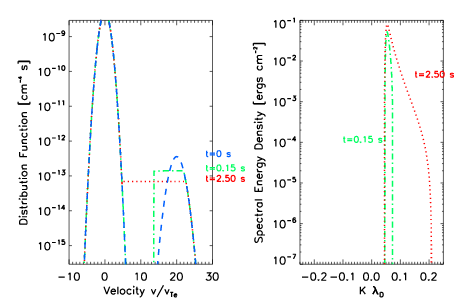
\includegraphics[width=0.75\columnwidth]{Images/L_wave_growth.png}
%     \caption[Langmuir wave distriburtion function and spectral energy density.]{Left: Evolution of distribution function (normalised by the electron thermal velocity $v_{Te}=V_e$) in time. The diffusive term in \ref{eq:dfdt} causes the bump-on-tail Gaussian to turn into a plateau, thereby eliminating the instability cause by the positive velocity gradient. Right: The spectral energy density of generated Langmuir waves, x-axis normalised to the Debye length $\lambda_D=\sqrt{\frac{\epsilon_0 k_B T_e}{e^2 n_e}}$. As time passes the spectral range of Langmuir waves increases. Each panel shows successive times of t=0.15s (green, dot-dashed line) and t=2.50s (red, dotted line). \citep[Figure taken from][]{Reid2014}.} %(Figure taken from \citeauthor{Reid2014} \citeyear{Reid2014})}
%     \label{fig:Lwavegrowth}
% \end{figure}

% \subsection{Wave-Wave Interaction}\label{Plasma Emission}
% Wave-wave interaction concerns the processes by which three types of waves interact. These are: transverse (T) waves, Langmuir (L) waves and ion sound (S) waves, and have the following, respective dispersion relations,
% $$ \omega=(\omega_p^2 +k^2c^2)^{\frac{1}{2}} $$
% $$ \omega \cong \omega_p + \frac{3k^2V_e^2}{2 \omega_p}$$
% $$ \omega = kv_s $$
% where $V_e$ is the thermal velocity of electrons in the plasma, $v_s$ is the ion sound speed and $k$ is the wave vector. Only transverse waves with $\omega > \omega_p $ can escape and thus a plasma emission mechanism is a process that generates these transverse waves. 

% As mentioned in Section \ref{characteristics}, Type III bursts have a harmonic structure associated with plasma emission at the plasma frequency and the second harmonic. Both of these transverse waves are formed in different three wave processes that will now be discussed.
% In a plasma, due to scattering from other wave modes and ions in the plasma, a wave mode can be changed from one to the other. This is expressed in the equation 
% $$ \sigma \rightleftarrows \sigma' + \sigma '' $$
% where $\sigma$, $\sigma'$  and  $\sigma ''$ represent different wave modes. Conservation of energy and momentum state,
% $$ \omega^{\sigma}(k)=\omega^{\sigma'}(k')+\omega^{\sigma''}(k'')$$
% $$ k=k'+k''$$
% where $ \omega^{\sigma}(k)$ is the frequency of a particular wave mode with the wave vector $k$. For Langmuir (L), ion sound (S) and transverse (T) wave modes the allowed processes are L+S$\rightarrow$L', L+S$\rightarrow$T,  T+S$\rightarrow$L,  T+S$\rightarrow$T' and  L+L'$\rightarrow$T. Of these L+S$\rightarrow$T,  L$\rightarrow$T+S are responsible for fundamental emission while harmonic emission is associated with the three wave process L+L'$\rightarrow$T.

% Originally \cite{Ginzburg1958} considered fundamental emission to be due to Langmuir waves scattering off of thermal ions in the plasma. It is now commonly accepted that the biggest cause of fundamental emission is due to the three wave processes of a Langmuir wave coalescing with an ion sound wave generated by L$\rightarrow$L'+S or when a Langmuir wave decays into an ion sound wave and an electromagnetic transverse wave. The process L$\rightarrow$T+S can be visualised as in Figure \ref{fig:Femission}. In solar radio physics it is often assumed that $k_L \gg k_T$, knowing this and that the wave vectors must satisfy $\mathbf{k}_L \pm \mathbf{k}_s = \mathbf{k}_T$ ($+$ for L+S$\rightarrow$T , $-$ for L$\rightarrow$T+S) implies $\mathbf{k}_s \approx \mp \mathbf{k}_L$ 

% \begin{figure}
% \centering
% 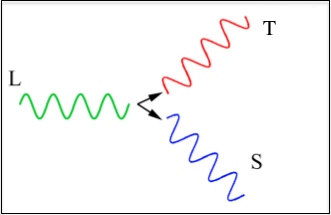
\includegraphics[width=0.5\columnwidth]{Images/Fundamental_emission_Lwaves.png}
% \caption[A three wave process of fundamental plasma emission L$\rightarrow$T+S]{A three wave process of fundamental plasma emission L$\rightarrow$T+S. A Langmuir wave decaying into an ion sound wave and an electromagnetic transverse wave at the plasma frequency. (Figure adapted from Solar (interplanetary) Radio Bursts: the Generation of Radio Waves,	an oral presentation by David Malaspina at the Jean Louis Steinberg International Workshop on Solar, Heliospheric and Magnetospheric Radioastronomy, November 2017)}
% \label{fig:Femission}
% \end{figure}

% Second harmonic emission occurs when two Langmuir waves coalesce in the process L+L'$\rightarrow$=T, shown in Figure \ref{fig:Hemission}. Conservation of momentum requires that $\mathbf{k}_L + \mathbf{k'}_L = \mathbf{k}_T$ and for second harmonic (H) generation, $k_T=k_H \approx \frac{\sqrt{3} \omega_p}{c}$. The phase speed $v_\phi$ of Langmuir waves is much less than $\frac{c}{\sqrt{3}}$ meaning that $k_L \gg k_T$ which results in $\mathbf{k}_L \approx -\mathbf{k'}_L$. This means that for a transverse wave at the second harmonic to be created, two Langmuir waves must coalesce almost exactly head on. These backward propagating Langmuir waves are generated: in the three wave processes of L+S$\rightarrow$L' and L$\rightarrow$L'+S; scattering off of thermal ions; and refraction at density inhomogeneities.
%  \begin{figure}

%      \centering
%      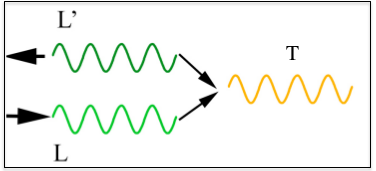
\includegraphics[width=0.5\columnwidth]{Images/Harmonic_emission_Lwaves.png}
%      \caption[Three wave process of second harmonic plasma emission L+L' $\rightarrow$ T]{Three wave process of second harmonic plasma emission L+L' $\rightarrow$ T. A Langmuir wave (L) and a backwards propagating Langmuir wave (L') coalesce to form a transverse wave (T) at $2 \omega_p$. (Figure adapted from Solar (interplanetary) Radio Bursts: the Generation of Radio Waves,	an oral presentation by David Malaspina at the Jean Louis Steinberg International Workshop on Solar, Heliospheric and Magnetospheric Radioastronomy, November 2017)}
%      \label{fig:Hemission}
%  \end{figure}

\section{Low Frequency Radio Wave Scattering}

\section{Radio Interferometry}
There are two limiting factors in modern-day optical astronomy, diffraction and atmospheric conditions. The latter has been overcome using advanced adaptive optics techniques or avoided entirely by putting telescopes in space. This leaves diffraction as a fundamental limit to the resolving power of any telescope.

Rayleigh's criterion states that for an object to be resolved, the maximum of its interference pattern must overlap the minimum of another. This leads to the mathematical relationship (assuming a circular aperature), $$\theta \approx 1.22 \frac{\lambda}{D}$$ where $\theta$ is the angular resolution of an object, $\lambda$ is the wavelength observed in and $D$ is the aperture diameter of the telescope. The Hubble Space Telescope, with a diameter of 2.4 m and observing in near IR therefore has an angular resolution of $\sim 0.05$ arcseconds. For a radio telescope observing 10 m waves to have the same resolution, ignoring atmospheric effects, it would need an aperture diameter of 41000 km. Building a single dish of this size is practically impossible. Fortunately, because radio waves are so large, they can be detected at multiple locations at great distances from each other and the original signal pieced back together. This idea forms the basis of radio interferometry.
The mathematical framework for this is \textit{slightly} more complicated than this simple view so to explain it the most fundamental radio interferometer, the two element interferometer, is described.

\begin{figure}
    \centering
    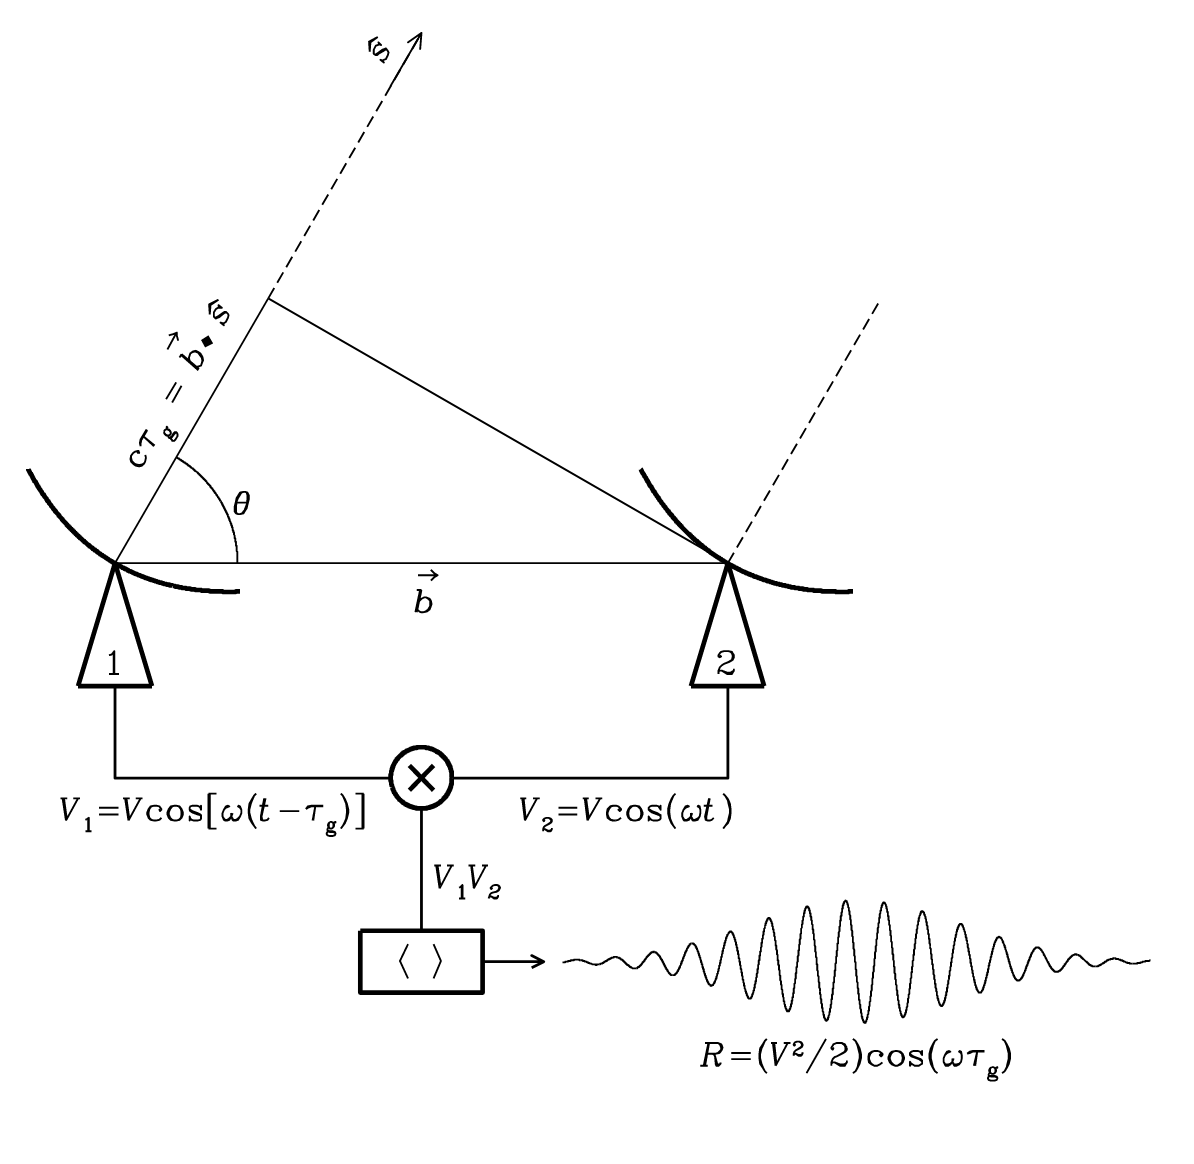
\includegraphics[width=0.5\columnwidth]{Images/2_elem_int.png}
    \caption[A two element interferometer]{A two element interferometer separated by a baseline $\overrightarrow{\Vec{b}}$. The signal from each antenna is correlated by first multiplying the two voltages then time averaging them.}
    \label{fig:2_el_int}
\end{figure}

Consider two radio antennae, 1 and 2, separated by a distance $\overrightarrow{\Vec{b}}$, this is the antenna baseline and is equivalent to the diameter of a classic telescope. A radio wave approaching the antennae from direction $\hat{\Vec{s}}$  will hit antenna 2 first then antenna 1 after a time delay of $\tau_g$ such that,
$$\tau_g = \frac{\overrightarrow{\Vec{b}} \cdot \hat{\Vec{s}}}{c} $$
where $c$ is the speed of light. The output from each antenna is a voltage $V_1 = V \cos{\omega(t - \tau_g)}$ and $V_2 = V\cos{\omega t}$. The total response, $R_c$ of the interferometer is the correlation or multiplication and time average of these two voltages, $\langle V_1 V_2 \rangle$. 
$$
R_c = \langle V_1 V_2 \rangle = \frac{V^2}{2} \cos{\omega \tau_g}
$$
Furthermore, if a 90$^\circ$ phase shift is added to the output of one antenna, the response becomes
$$
R_s = \langle V_1 V_2 \rangle = \frac{V^2}{2} \sin{\omega \tau_g}
$$
A complex visibility can be defined as the complex sum of the two responses $V(\hat{\Vec{s}}) = R_c - iR_s$. Using Euler's formula, the complex visibilty of an extended source is given by:
\begin{equation}
\label{eq:complex_vis}
V(\hat{\Vec{s}}) = \int I(\hat{\Vec{s}}) \exp{(-i \omega \tau_g)} d\Omega = \int I(\hat{\Vec{s}}) \exp{(-2 \pi i \frac{\overrightarrow{\Vec{b}} \cdot \hat{\Vec{s}}}{\lambda}}) d\Omega
\end{equation}
where $I$ is the sky brightness distribution. In more conceptual terms, the complex visibility is the Fourier transform of the sky brightness distribution.

Equation \ref{eq:complex_vis} can be rewritten as a function of the \textit{uvw} coordinate system and using the directional cosine coordinate system for source position on the sky.

% their phase information can be recorded. Thus, multiple, smaller radio antenna placed at great distances will obtain the same resolution as a single dish. such that $\overrightarrow{\Vec{b}} \cdot \hat{\Vec{s}} =b\cos \theta$
\begin{equation}
\label{eq:complex_vis_uvw}
V(u,v) = \int I(l,m) \exp{(-2 \pi i (ul + vm))}\ dl\ dm
\end{equation}

The coordinate system commonly used throughout radio interferometer is the \textit{l,m,n} or directional cosine coordinate system. This determines a position on the sky in terms of the direction cosines to that position. Here \textit{l,m,n} are defined as
$$ l =  \cos \delta  \sin \Delta \alpha, \ 
 m = \sin \delta \cos \delta_0 - \cos \delta \sin \delta_0 \cos\Delta \alpha, \ 
 n = \sqrt{1-l^2-m^2}$$
where $\delta, \delta_0$ are the declinations of an object and the phase centre, respectively, and $\Delta \alpha = \alpha -\alpha_0$ is the difference between the right ascension of the object and phase centre (direction of the primary beam).

Baselines in radio interferometry are described using the \textit{uvw} coordinate system defined as
\[
\begin{bmatrix}
    u \\
    v \\
    w
\end{bmatrix}
=
\dfrac{1}{\lambda}
\begin{bmatrix}
    \sin H       & \cos H & 0 \\
    -\sin \delta \cos H       & \sin \delta \sin H & \cos \delta \\
    \cos \delta \cos H       & -\cos \delta \sin H & \sin \delta
    

\end{bmatrix}
%
\begin{bmatrix}
    B_x \\
    B_y \\
    B_z
    

\end{bmatrix}
\]
Here, $H$ is the hour angle of an object, $\delta$ is its declination, $\Vec{B}=(B_x, B_y, B_z)=(x_2-x_1,y_2-y_1,z_2-z_1)$ is the baseline or distance between two antennae and $\lambda$ is the wavelength of the radio waves being observed.
\subsection{Beam-forming}
\label{sec:beamform_theory}
In its most simple terms, beamforming  means pointing a phased array in a particular direction. It involves correcting for phase difference between the ``phase centre" of the beam and the position of the source of interest for each baseline and then summing it all together. % Beamforming in a LOFAR station is done by the RSP boards (section \ref{sec:rsp}) in a matter of seconds however, in order to utilise TBB data (section \ref{sec:tbb}), this must be done in post processing which can take considerably longer.%In practice this turns out to be a bit of a pain, not only because you quickly get lost in the various coordinates and notation needed but also it drastically increases the number of FTs you need to do, which slows any and all processing right down. 
In order to beamform, one must account for the phase difference between the phase centre (where the beam is physically pointing) and the source (at an angular coordinate of \textit{(l,m)} with reference to the phase centre). As above, this phase difference for a baseline pq is given by, 
$$\kappa_{pq} = 2\pi(u_{pq}l+v_{pq}m+w_{pq}(n-1))$$
In order to correct for the phase difference and steer the beam, data for baseline pq is multiplied by the complex weight $e^{-i\kappa_{pq}}$, this is repeated for all baselines and finally all data is summed.

\section{Thesis Outline}